%!TEX root = ./Structure_rapport_final.tex


% Resitue le sujet dans une problématique générale ;
%  -restitue le sujet dans un cadre de gestion plus global
% - doit également justifier le bien-fondé de l’étude en fonction des demandes
% • Donne les objectifs qui ont été fixés pour répondre à la question posée ;
% • Présente la démarche qui va permettre de répondre aux objectifs.


% \subsection{Présentation des milieux marins profonds}
% - milieu peu connu, écosystème particulier --> communauté sur laquelle on travaille 
% - particuliarité des canyons 
% - Rôle de ces espèces dans les chaines trophiques (plus faibles maillons et MM/oiseaux)
% - communauté de poisson méso-bathy pélagiques 

% \subsubsection*{Présentation de l'environnement}
Deep-sea is the largest marine habitat of Earth, and represents 95\% of ocean's volume \citep{danovaro2017,salazar2016}. From a biology perspective, deep-sea encompasses everything beneath euphotic (or epipelagial) zone, where the solar radiations are too low and precludes photosynthesis \citep{baker2020,danovaro2017,salazar2016} (see Figure~\ref{fig:dsl}). Between 200 to 1000m deep (mesopelagic zone), light fades and temperature decreases, because solar luminance is absorbed exponentially in upper sea layers \citep{reynolds2001}. From 1000 to 4000m deep (bathypelagic zone), no sunlight remains and the habitat is pitch-black; salinity and temperature are stable (between -1.8 to 2°C), and pressure keeps on increasing by 1 atm every 10m \citep{danovaro2017}. 

\begin{figure} [!htbp]
	\begin{center}
		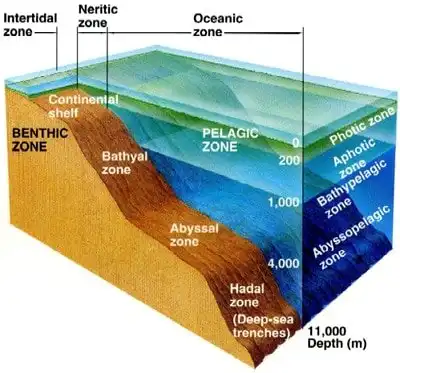
\includegraphics[width=0.5\textwidth]{sea_layers.png}
	\end{center}
	\caption[Petite légende]{Sea layers along depth, from \citep{fig_deep_sea}}
	\label{fig:dsl}
\end{figure}

Despite those extremes conditions, and low rate of food supply deep-sea is far from being lifeless. In fact, deep-sea is considered to be the largest biome of the Earth, and contains 70\% of ocean's microbial cells and 60\% of its heterotrophic activity, playing a crucial role in biogeochemical cycles \citep{salazar2016}. Studies from \citet{grassle1992,parkes1994,todo2005} shown that life could be found everywhere in the deep-sea, with remarkably high and stable diversity. With first studies launched in the 60's, less that 0.0001\% of the area has been investigated so far and and this whole habitat remains understudied \citep{danovaro2017,richards2019}. Thus, deep-sea remains the most unknown biome of the planet with estimated 10 million species that are yet to discover \citep{danovaro2017,grassle1992}. In particular, data are lacking to evaluate the impact of climate change on the biodiversity of the largest reservoir of biomass, mainly because exploring deep-sea is difficult and requires specific tools, such as rovers \citep{danovaro2008,danovaro2014}. Firstly, deep-sea were regarded as a ore reservoir, where manganese and other metal deposits could be found and extracted, or even as a dumping site for nuclear wastes \citep{baker2020,gillet2013,halfar2002}. But since past decades, capacity of exploration of the deep-sea expanded spectacularly, allowing seachers to discover more about the depth of the oceans \citep{danovaro2014}.

In particular, continental margins, which separates continental shelf from abyssal plains are investigated, because their heterogeneous topography implies varied habitats and hydrodynamics, with impacts on the whole food chain \citep{danovaro2009,fernandez-arcaya2017}. Along continental margins, deep-sea canyons, that incises the edges of continental shelf, appears to be ``biodiversity hotspots'' for pelagic life, in terms of diversity and abundance \citep{aissi2012,danovaro2009,gillet2013,robertson2020}. Because they are the main conduits transfering organic matter and sediments from rich and productive shallow shelf to the low-nutrients deep-sea, canyons constitues peculiar habitats, with evidences of an important biomass and diversity of benthic organisms \citep{canals2006,danovaro2009,leo2012}, but also of fishes assemblages \citep{sion2019,stefanescu1994} around them. Indeed, canyons locally displays higher nutrients concentrations than in adjacent areas, due to down-welling currents creating a funnel-effect \citep{fernandez-arcaya2017}. Thus, primary production is enhanced, and makes canyons favourable habitats for filters and suspension feeders \citep{fernandez-arcaya2017,sion2019}, but also for low trophic levels organisms, such as euphausiids, shrimps, squids and meso- and bathypelagic fishes \citep{aissi2012,gaskett2001,pusch2004}. Abundance of nutrients and preys attracts top predators (cetacean, sharks, large pelagic), some of them being only encountered in those habitats \citep{aissi2012}. Specialized habitats, deep-sea canyons displays high level of endemism \citep{danovaro2009,danovaro2017}, are source of rich marine biodiversity and many services \citep{fernandez-arcaya2017}. Among those, canyons play a role in sustaining deep-sea food webs through the transport of nutrients, providing habitat for nursery and refuges \citep{fernandez-arcaya2017}. \citet{company2008} suggests that by those services, canyons enhance recruitement of commercialised species, and thus, may mitigate the effect of their overexploitation. Therefore, canyons can be described as ``keystone structures'', as an interface between productive continental shelf and deep-sea, with evidence of their benefits and supports for fisheries \citep{company2012,fernandez-arcaya2017}.

\subsubsection*{Présentation des poissons méso et bathy pelagiques}
Meso- and bathypelagic fishes are found abundantly in every ocean, except Arctic, and are the dominant zooplankton consumers in most oceans, playing a key role in trophic networks \citep{davison2015,salvanes2009}. Living between 200-1000m (mesopelagic) and over 1000m (bathypelagic) deep, those deep-sea fishes displays very high biomass, estimated to be around ten billion tonnes in total \citep{garcia2021,gjoesaeter1980,richards2019}. Though, abundance of those fishes varies along depth and daytime, because most of them perform vertical diel migration to feed on shallower depth during night, and abundance's estimation can be biaised by sampling time \citep{catul2011,gaskett2001,garcia2021,pusch2004,salvanes2009}. Performing migrations, meso- and bathypelagic fishes ensure biogeochemical cycling through respiration and excretion but also when predated by carnivorous \citep{garcia2021,spitz2019}. Because of their ubiquity, their biomass and the high efficiency of energy transfer from phytoplankton ( respiring 10\% of the primary production),  meso- and bathypelagic fishes play an important part of the biological pump \citep{garcia2021,spitz2019}.
Meso- and bathypelagic fishes shows adaptations to their environment: sensitive eyes, dark body and ventral light organs (photophores) to match their low-light habitat and reduced metabolic rates to lower oxygen consumption in poorly oxygened waters \citep{salvanes2009}. Photophores have a role in camouflage, courtship behavior, with differents patterns between males and females, and are also species specific which helps identification \citep{paitio2020,salvanes2009}. 

In terms of life history, \citet{childress1980} and \citet{salvanes2009} observed some differences bewteen meso and bathypelagic fishes. The first are characterised by a relatively small size (2-15cm long), slow growth and have a rather long (short d'après Salvanes??) life span, with repeated reproduction and high reproductive rate. Conversely, bathypelagic fishes tends to have larger size, rapid growth but short lives and late reproduction, that seems to occur during the last year of their life. The mesopelagic communities are dominated by Myctophidae family, in terms of abundance, diversity and biomass, and represents at least 20\% of the whole oceanic ichtyofauna \citep{catul2011,kozlov1995,pusch2004}. (peut-être à mettre dans matériels et méthodes plutôt ?)


% \subsubsection*{Zoom sur le gdG}

If several studies focused on exploring deep-sea fish diversity near seamounts, mid-ocean ridges or in abyssal depths \citep{cook2013,sutton2013}, very little is known about meso- and bathypelagic species inhabiting deep-sea canyons \citep{kenchington2020}. Not only does this lack of information precludes comparisons between canyons, hence limiting the chances to highlight endemism, but it also restrains reliability of ecosystemics and biogeochemistry models \citep{davison2015,kenchington2020}. Indeed, given the essential role of those fishes in food webs, linking the epipelagic organic matter they feed on to the deep-sea, and in biogeochemical cycling, better knowledge of species constituing this fundamental compartment is crucial \citep{davison2015,gaskett2001}. Furthermore, considering how important canyons are for fisheries and carbon sequestration, knowing more about the communities inhabiting them is crucial to ensure sustainability of ecosystems and provided services, through marine management and conservation \citep{fernandez-arcaya2017,vandenbeld2017a}.

Studied here, the continental margin of the Bay of Biscay covers nearly half of France's Atlantic EEZ (Exclusive Economic Zone) and is incised by about 135 canyons \citep{bourillet2006,spitz2019,vandenbeld2017} (see Figure~\ref{fig:bbm}). If proven to be rich in cold-water coral reefs, the largest part or the area remains poorly explored, especially deep-pelagic communities \citep{garcia2021,vandenbeld2017a,webb2010}.

\begin{figure} [!htbp]
	\begin{center}
		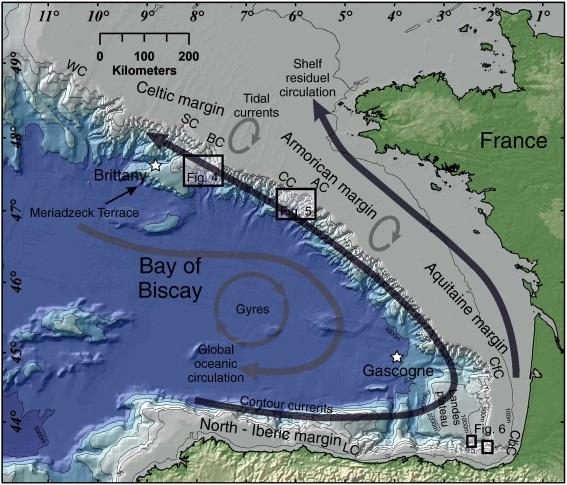
\includegraphics[width=0.6\textwidth]{Biscay_Bay_map.png}
	\end{center}
	\caption[Petite légende]{Location of the studied area, from \citep{mulder2012}}
	\label{fig:bbm}
\end{figure}

Hence, the aim of this work is developp knowledge of communities inhabiting deep-sea canyons of the Bay of Biscay. To do so, functional approach seems relevant because it overrides limitations that taxonomic approach have and allows generalisation of the method. Defining functional niches of canyons communities will help understanding how they share resources and which are the functions ensured. The main hypothesis is that species occupying similar functional niches would be considered as being redundant from a functional perspective, whereas species displaying very different functional niches would be segregated. 

% \subsection{Axes pour une meilleure connaissance de ces écosystèmes}
% - comment les espèces se partagent les ressources (bcp d'études déjà terrestres)
%          --> focus sur cette communauté particulière qui est pour l'instant peu connue

% - 2 approches possibles: 
% 		- espèce-centrée : seule ou en compétition --> mais limitant pour la comparaison entre écosystèmes différents. 
% 		- communautaire : certaines espèces sont-elles redondantes ? Plusieurs espèces
% occupent la même niche en cas de chevauchement, occupent la même niche fonctionnelle. Se focaliser
% sur les fonctions plutôt que sur l'espèce. --> Permet une généralisation de la méthode et une comparaison entre écosystèmes
% 		- Individus appartenant à la meme niche peuvent être considérés comme appartenant
% à la même boîte fonctionelle. 
% ==> Caractériser un écosystème par les fonctions qu'ils présentent plutôt que par ses espèces

% \subsection{Présentation de la démarche et des objectifs}
% - mieux connaitre ces communautés à travers les niches qu'elles occupent dans les écosystèmes
% - caractériser leurs niches trophiques, comportements, habitats, sensibilité des espèces, 
% particularité des espèces, voir les avantages de partager les niches 
% - Envisager une approche universelle, permettant la comparaison d'écosystèmes

% - Hypothèses: chevauchement de niches entre les espèces, entrainant de la compétition entre les espèces ayant des fonctions similaires, ou ségrégation, où les espèces
% utilisent des ressources distinctes et ont des fonctions différentes

